\section{Results \& Analysis}\label{sec::results}

\subsection{Comparing Performance}
We seek to evaluate the overhead of each language's concurrency framework. Therefore, we present the normalized speedup as a function of the number of threads for each benchmark implementation from 1 to 8 threads in Figure~\ref{fig:speedup}. 
\begin{figure}
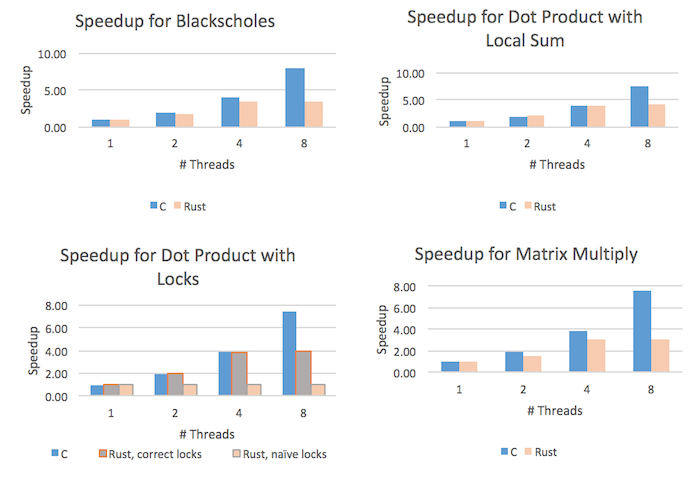
\includegraphics[scale=0.4]{speedup_benchmarks}
\caption{Speedup in each language}
\label{fig:speedup}
\end{figure}

\begin{figure}
\centering
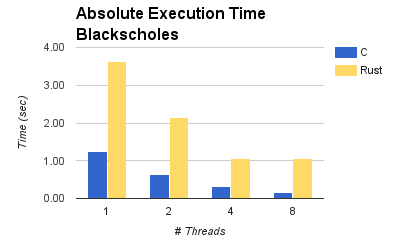
\includegraphics[width=0.45\textwidth]{blackscholes_abs.png}
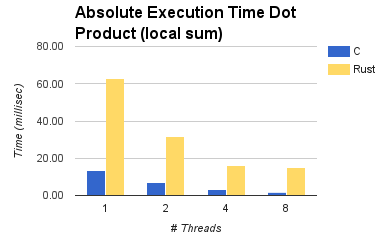
\includegraphics[width=0.45\textwidth]{dot_product_local_abs.png}
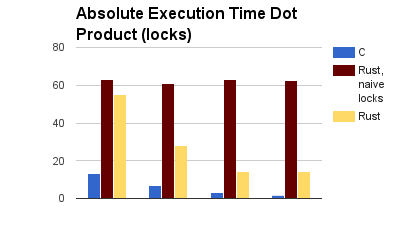
\includegraphics[width=0.45\textwidth]{dot_product_locks_abs.png}
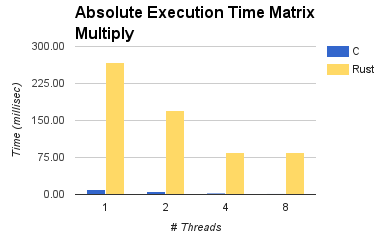
\includegraphics[width=0.45\textwidth]{mm_abs.png}
\caption{Execution of blackscholes for 1 to 8 threads on a reference Linux 8 core machine.}
\label{fig:absolute_time}
\end{figure}

The speedup ideally scales with the number of threads. One can see that C very nearly achieves this in every benchmark. Rust keeps up best in both implementations of dot product, fairly well in blackscholes, and less so in matrix multiply.

Figure~\ref{fig:absolute_time} displays our absolute execution times recorded for the four benchmarks. Generally speaking, C still dominates Rust by a relatively wide margin in terms of execution time. Consequently, there is definitely a performance cost associated with using Rust instead of C. In spite of this, Rust's execution time halves every time the number of threads is doubled for 1 through 4 threads, which corresponds to the doubling of speedup as observed in Figure 1.

A striking result from our Sniper simulations is that at 8 threads, on an 8 core machine, Rust lags behind C egregiously. Figure~\ref{fig:instr_load} shows that this is due to a workload imbalance that only afflicts our Rust benchmarks. One can see that for each Rust benchmark, core 0 is largely idle while another core takes on twice the work as the others and thus slows down the entire program. Hence our slowdown at eight threads in Sniper.

We investigated this discrepancy further by running the Rust blackscholes benchmark on an 8-core physical machine to see if this problem was merely an artifact of the Sniper simulator. Figure~\ref{fig:baremetal} shows that on a physical machine, normalized speedup continues to improve at eight threads, contradicting our simulator results from Figure~\ref{fig:speedup}. Admittedly, because we were unable to isolate the parallel region of interest on our physical machine, we see diminishing returns in speedup as the number of threads increases, as described by Amdahl's Law. Still, we have conclusively determined that the Sniper scheduler is giving erroneous results for Rust at eight threads due to some issue with its scheduler. It is interesting that this problem in Sniper occurs only with our Rust programs, not our C programs. Nevertheless, because of this simulator error, we feel it is best to ignore the data point for speedup at eight threads in Figure~\ref{fig:speedup}.
\begin{figure}
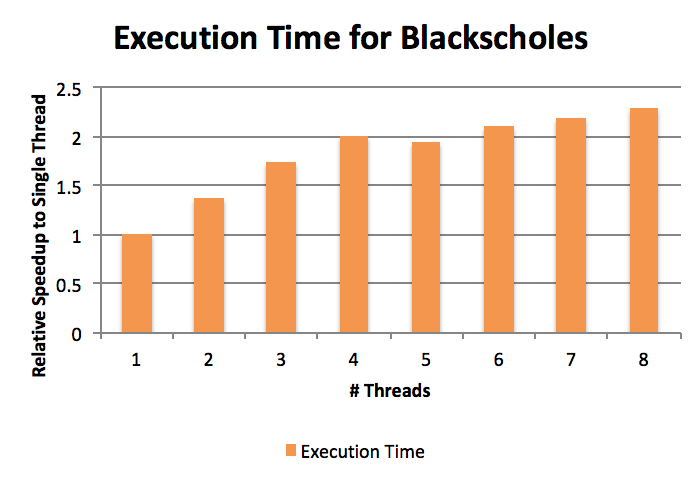
\includegraphics[scale=0.7]{relative_speedup}
\caption{Execution of blackscholes for 1 to 8 threads on a reference Linux 8 core machine.}
\label{fig:baremetal}
\end{figure}

\begin{figure}
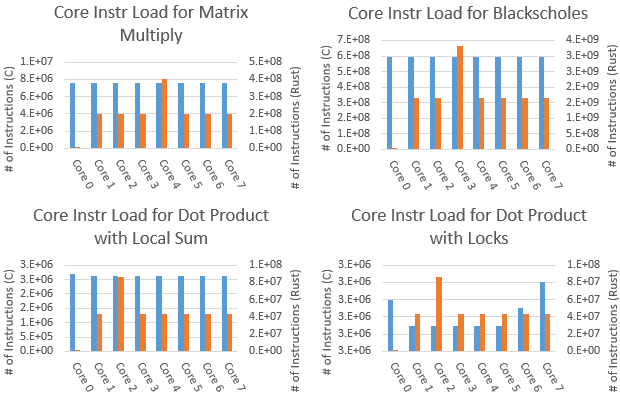
\includegraphics[scale=0.4]{instr_benchmarks}\\
\caption{Instruction load per core at eight threads running in Sniper}
\label{fig:instr_load}
\end{figure}

Additionally, a compelling ``gotcha'' we uncovered was the unexpected slowdown of the Rust dot product benchmark when unwrapping and modifying locked data in one line. To ensure memory safety, the Rust compiler emits synchronization code (as well as other memory management code e.g. destructors) around accesses to objects of type \texttt{Mutex<T>}. In our dot product benchmark's original implementation, the result of the parallel dot product computation was used as an rvalue for an addition operation on a synchronized variable (see Listing~\ref{list:rvalue}).

\begin{lstlisting}[caption={Rvalue used in serialized add},label=list:rvalue]
*dotprod_shared.lock().unwrap() +=
			dot_prod(&x_shared, &y_shared, start, end);
\end{lstlisting}

This unexpectedly serialized the computation of the rvalue as well such that no benefit came from parallelization, as shown by the flat line labeled "naive locks" in Figure~\ref{fig:speedup}. Ideally, the compiler would compute the rvalue before attempting to unlock the lvalue so that the program would not be serialized. This problem was solved by expressing the above in two lines, as shown in Listing~\ref{list:2line}.
\begin{lstlisting}[caption={Rvalue used in serialized add},label=list:2line]
let thrdsum = dot_prod(&x_shared, &y_shared, start, end);
*dotprod_shared.lock().unwrap() += thrdsum;
\end{lstlisting}

\subsection{Comparing Ease of Implementation}
Although Rust's ownership system ensures memory safety and synchronization of data, there exists a learning curve that must be overcome. As newcomers to the Rust language, we had difficulties complying with the ownership system at first. However, over time we began to appreciate Rust as it forces the programmer to consider the safety of their code. In the same vein, Rust forces the programmer to think about parallel memory safety. However, there are still some annoyances about Rust that can, at times, make implementing a simple algorithm difficult.

For example, we found Rust's insistence on avoiding any possibility of a data race to be cumbersome at times. In the matrix multiplication benchmark, each thread is given exclusive access to a section of a shared data structure. Rust prevents the data structure from being shared across multiple threads for fear of a data race, even though accesses are mutually exclusive in our algorithm. In C, this is of course not a problem, but we found Rust's strictness to be a hindrance.

We looked to other threading libraries as a way of circumventing this issue. We settled upon \texttt{crossbeam}'s scoped threads as a way of statically specifying the portion of the output matrix that each thread could mutate. This way, we could implement our algorithm as we did in C, and the Rust compiler could be guaranteed that accesses to regions of the data structure were mutually exclusive. Initial debugging of this issue proved to be painful because of nebulous compiler errors and our lack of Rust expertise, but integration of the library to implement the fix was easy thanks to Rust's \texttt{cargo} package manager.

Overall, we found that in this instance, writing safe Rust code was more of a hassle than beneficial, since we knew in advance that our chosen algorithm was thread-safe. In this case, it may have been appropriate to use Rust's \texttt{unsafe} tags to surround concurrent accesses to the shared output matrix, but in retrospect we feel it was worthwhile to see the lengths one would need to go to make this algorithm compliant with Rust's ownership rules. Our conclusion is that while it is possible to make it apparent to the compiler that our algorithm is thread-safe, there is no value in doing this if we have already verified that this is so on our own. Rather, the real value of Rust in this case is that it forced us to prove this to ourselves before moving forward.